\subsubsection{Layers vs no layers}
In this experiment we tried to figure out whether or not stacking an LSTM would help increase the performance of the network. The idea was that adding this extra non-linearity would make it able to find better patterns in the structures of these proteins and thereby get better results. The results show that simply stacking them without anything else does not provide any kind of improvement, quite the opposite in fact. The resulting Spearman's rho values of $0.474$ for the single-layer and $0.400$ for the double-layered models attest to this. One possible explanation for this could be that the model begins overfitting on the data when stacked in this way. It is interesting to note that while the 1-layer model gets a better Spearman correlation score, its next token prediction accuracy is slightly worse. Considering the fact that a 2-layer LSTM takes roughly twice as long to train as a 1-layer LSTM, stacking them like this does not seem like a good way to increase the performance of an LSTM for this task.

\subsubsection{Dropout vs. no dropout}
In this experiment, we tested whether adding dropout between the layers of a stacked LSTM would help increase the robustness of the network. Now, considering the results from the previous experiment, we weren't expecting a significant improvement over the baseline single-layer model. The results were very interesting however; the next token prediction accuracy was basically the same, with only a $0.01\%$ difference on the test set. Meanwhile, the Spearman correlation score improved quite significantly, scoring $0.518$, compared to the $0.400$ of the 1-layer model. This may be because the dropout forced the network to learn a better general representation of the structure, rather than learning a few signs that may not always be there. This model takes a slightly shorter time to train than the network without dropout. Because of this, adding dropout between layers of a stacked LSTM seems to be a great way to increase both the performance and robustness of the network.

\subsubsection{Feature size}
It is to be expected that reducing the number of features a model can use will limit how much it can learn. For this experiment we decided to see whether the increased amount of data a smaller model can be trained on due to the increased speed would make up for that lack of features. For reference, the smallest model at $256$ hidden features trained for $60$ epochs, while the largest at $1024$ hidden features only trained for $10$. The model with $512$ features trained for $30$ epochs. We expected that there would be some middle ground between speed and the number of features, but actually saw that increasing the features was a boost to performance in all the cases we tested. Since we were limited by hardware, going over $1024$ features was not possible. An interesting note is that there is a very large difference between how the next token predictions actually look. It seems like the $256$ model has not learned much more than predicting which amino acids are the most common. Meanwhile, the larger $1024$ model seems to have learned significantly more about the structure of the protein and varies its predictions much more. An example of this can be seen in Figure ~\ref{fig:predictions}. This can also be seen in the Spearman correlation scores, in which the $1024$ model scores significantly higher than the others.


\begin{figure}[!ht]
  \centering
  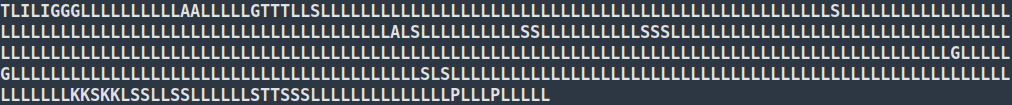
\includegraphics[width=0.49\linewidth]{latex/imgs/256_prediction.png}
  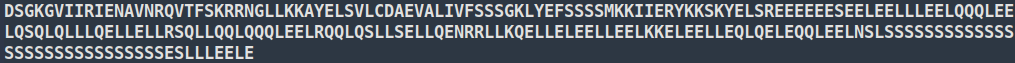
\includegraphics[width=0.49\linewidth]{latex/imgs/1024_prediction.png}
  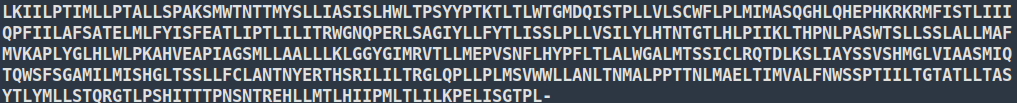
\includegraphics[width=0.49\linewidth]{latex/imgs/256_labels.png}
  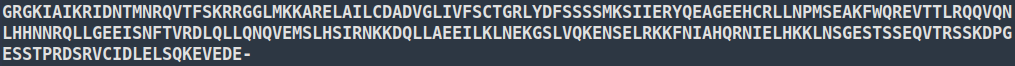
\includegraphics[width=0.49\linewidth]{latex/imgs/1024_labels.png}
  \caption{Example of how different the predictions look. Left column uses the $256$ feature model, right column uses the $1024$ feature model. The model predictions are in the top row, the corresponding labels are in the bottom row.}
  \label{fig:predictions}
\end{figure}

\subsubsection{Learning rate}
We observed quite early on that there was a very large variance in the loss values during training, and that the variance increased significantly as training went on. Thus, for this experiment, we used a learning rate scheduler to hopefully combat this phenomenon. An example of this variance can be seen in Figure ~\ref{fig:loss_var}. The results were very unexpected, however. First of all, the variance in loss did not decrease significantly, though it did seem to cause slightly fewer large outliers. The model that did not have a learning rate scheduler actually performed significantly better, to the point where it is the highest-scoring of the final models, with a Spearman correlation of $0.605$. Meanwhile, the counterpart with a scheduler only scored a $0.474$. We do not think that we can draw to the conclusion that this result means that using a scheduler makes the model perform worse. We think that the reason the model without scheduling performed so much better was that the scheduling was too aggressive. It is a tough parameter to adjust however since it requires you to know roughly where it is necessary to lower the learning rate for better results. As we see in the next experiment however, the scheduler may actually have caused the model to perform significantly better in the minloss version, however.

\begin{figure}[!ht]
  \centering
  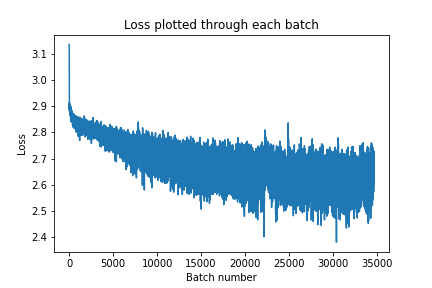
\includegraphics[width=0.5\linewidth]{latex/imgs/loss_log_1_layer_no_schedule_512.png}
  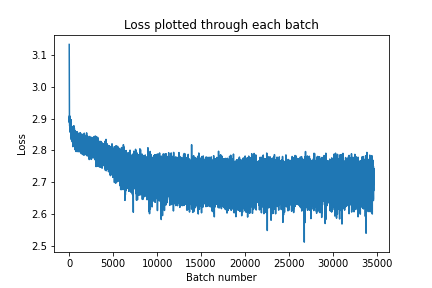
\includegraphics[width=0.5\linewidth]{latex/imgs/loss_log_1_layer_with_schedule_512.png}
  \caption{Example showing the increasingly large variance while training. The plot on the right uses a learning rate schedule where it multiplies the learning rate by $0.2$ every $5$ epochs.}
  \label{fig:loss_var}
\end{figure}

\subsubsection{Minimum loss model vs last model}
Due to the large variance in the loss values, there are a few batches during training in which the model has significantly better loss values than the average. This led us to save the best of these models, to try and see how well they performed compared to the final models. The results were quite interesting, to say the least. In only two of the six models, we trained for experiments did the minloss model performs worse than the final models. These two models were the $256$ feature model with scheduling, and the $512$ feature model without scheduling. In both cases the Spearman correlation was only slightly worse, however; decreasing by $0.011$ and $0.013$ respectively. The rest of the models experienced moderate to significant improvements in their Spearman correlation scores however, with the largest jump increasing the score by $0.124$. We can only guess as to why two of the models performed worse, but we have a hypothesis that the reason the other models saw such a large increase was helped along by the learning rate scheduler.